\begin{frame}
	\frametitle{Forme générique du langage auteur}
	\framesubtitle{Le langage auteur : quel but ?}

	\begin{block}{Critères pour le langage auteur}
		\begin{itemize}
			\item Facile d'utilisation
			\item Extensible
			\item Fonctionnement par balises
		\end{itemize}
	\end{block}

	\begin{block}{Syntaxe d'une balise}
		\begin{itemize}
			\item Nom
			\item Champ de méta-données optionnel
			\item Paramètre principal optionnel
		\end{itemize}
	\end{block}
\end{frame}

\begin{frame}
	\frametitle{Forme générique du langage auteur}
	\framesubtitle{Les balises}

	\begin{block}{Portée d'une balise}
		L'effet de la balise perdure jusqu'à qu'elle rencontre
		une balise plus importante qu'elle.
	\end{block}

	\begin{block}{Forme d'une balise}
		\texttt{\$sonNom (ses méta-données) son paramètre principal}
	\end{block}
\end{frame}

\begin{frame}
	\frametitle{Spécification du vocabulaire}

	\begin{itemize}
		\item Définit le vocabulaire et la sémantique
		\item Est donné sous la forme de documents XML
	\end{itemize}

	\begin{block}{Exemple}
		<Balise
		\ \ \ \	nom = «tox» priorité = «50» \\
		\ \ \ \	concerne = «nom du produit concerne» \\
		\ \ \ \	porte = «consignes de sécurité associées» \\
		\ \ \ \	detecte\_occurrence= «bulle» \\
		\ \ \ \	cree\_bulle\_avec= «contenu» \\
		\ \ \ \	table\_associée = «Produits Toxiques» \\
		\ \ \ \	references\_croisée = «oui» \\
		\ \ \ \	nom\_xml= «prodtox» /> \\
	\end{block}
\end{frame}

\begin{frame}
	\frametitle{Fonctionnement interne d'EadGen}

	\begin{figure}
		\centering
		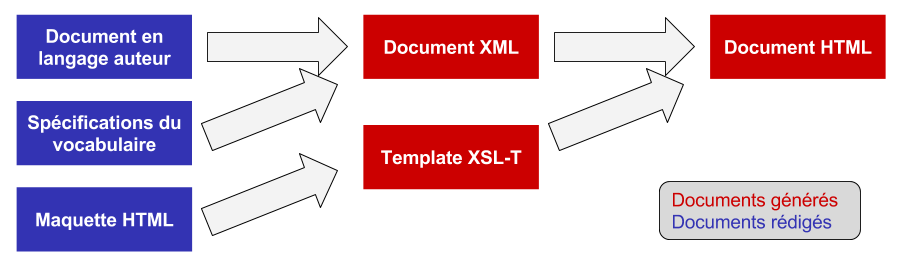
\includegraphics[scale=0.32]{resources/fctEadgen.png}
		\caption{Documents générés par EadGen}
	\end{figure}
\end{frame}

